%% muonDetectionSystem.tex
%%

%% ==============
\chapter{The muon detection system}
\label{ch:The muon detection system}
%% ============== 
  The need for low background rates at the main detector requires for a good knowledge of background sources. Despite magnetic reflection and wire electrodes, cosmic ray and particularly cosmic muon induced background may be an issue for the KATRIN experiment. To gather and asess muon related data, scintillator modules have been installed at both the monitor spectrometer and the main spectrometer. While the monitor spectrometer is equipped with only two rather small modules, at the larger main spectrometer, 8 modules have been installed at different positions enabling the user to cover different regions of the vessel. This freedom is enlarged by installing the detection system on three independently movable trolleys.
  The modules have been connected to the DAQ one trolley per card, meaning modules one and two connect to card three, modules 3 through 5 to card six and modules 6 through 8 to card nine (\ref{tab:connectionsModulesCards})
  \begin{table}
	\label{tab:connectionsModulesCards}
  	\centering
  	\begin{tabular}{| l | c c | c c | c c | c c |}
  	\hline
  		Module	& 1A	& 1B	& 2A	& 2B	& 3A	& 3B	& 4A	& 4B 	\\
  		Card	& 3	& 3	& 3	& 3	& 6	& 6	& 6	& 6	\\
  		Channel	& 0	& 14	& 3	& 7	& 0	& 14	& 3	& 7	\\
  		\hline \hline
  		Module	&5A	& 5B	& 6A	& 6B	& 7A	& 7B	& 8A	& 8B	\\
  		Card	& 6	& 6	& 8	& 8	& 8	& 8	& 8	& 8	\\
  		Channel	& 9	& 23	& 0	& 14	& 3	& 7	& 9	& 23	\\
  		\hline
  	\end{tabular}
  	\caption{Assignment of module sides to cards and channels}
  \end{table}
  All connections from modules to DAQ are made of coaxial cabling of equal length. This ensures comparable timestamps which are assigned only after the analogue signals arrive at the DAQ. High voltage is provided by two supplies, one on the east and one on the west side of the main hall.
  All devices of the muon detection system are connected to two multiplugs that are both overcurrent protected and feature mains filters. These multiplugs have been modified \ref{fig:multiplug} to connect to a ground other than the outlet's. To ensure a common potential for all of the devices and the surrounding appliances this connection was made to the trough below the main vessel.
  
  \begin{figure}
  \centering
  \label{fig:multiplug}
  	\includegraphics[width = 0.4 \textwidth]{graphics/setup/multiplug.pdf}
  	\caption{Added extension of the earthing contact to connect to any ground needed}
  	
  \end{figure}
\todo{insert photograph of multiplug}


%% DAQ.tex
%%

%% ==============
\section{Data aquisition crate}
\label{ch:DAQ}
%% ==============
The Data acquisition crate, short DAQ, is the central part of event recording and by that the interface between hardware muon modules and software based ORCA machine. It features first and second level trigger cards that are described in detail in the following chapters. The linux based system runs on an external hard drive connected to the second level trigger card via USB. Here, a screen and keyboard can be connected for network setup, then, access via ssh is possible. The DAQ can be connected to and controlled by the ORCA software.
  %% ===========================
  \subsection{First level trigger cards}
  \label{ch:DAQ:sec:FLTs}
  %% ===========================
  The FLT cards directly receive the signal output of the photomultiplier tubes via coaxial cabling. They then do first parts of data analysis to reduce data flow to the ORCA machine. In this case, only events with occur simultaneously on both sides of any module are passed on. This reduces the rate from \todo{look up non veto rate} to around \SI{250}{\hertz}. The FLT cards are made up of a large main card and a smaller connector card. 
  %% ===========================
  \subsection{Second level triger cards}
  \label{ch:DAQ:sec:SLTs}
  %% ===========================
  Only one second level trigger card is installed on each DAQ. all the Signals from the FLT cards are stacked here and passed on to the the ORCA machine. Networking runs directly through the SLT card. Other connections, such as USB, a display port, and also the CAT 5 connectors for synchronisation to a clock can be attached here.

  %% OrcaControl.tex
%%

%% ==============
\section{Orca control}
\label{ch:OrcaControl}
%% ==============
    ORCA is the central software for data acquisition. It is able to control lots of different devices via almost any kind of interface, while it is easiest to use ethernet connections. 

    %% ===========================
    \subsection{Software Gains and Thresholds}
    \label{ch:OrcaControl:sec:SoftwareGainsThresholds}
    %% ===========================
    
    
    %% ===========================
    \subsection{Run control}
    \label{ch:OrcaControl:sec:RunControl}
    %% ===========================
    Runs are the basic element of data storage, every time data is recorded, a run is created. Inside every run can be a number of subruns, at least there is one, that will in turn contain data classes such as KaLi::KLVetoEvents, the most used event class in case of the muon modules.
    
    %% ===========================
    \subsection{File handling}
    \label{ch:OrcaControl:sec:FileHandling}
    %% ===========================
    All runs created are first saved to the local disc of the Mac machine. Sorting in folders for year and month is applied to quickly find what zou are looking for. They are then uploaded to servers of the IPE via cronjobs, a feature of the Linux based MacOS. Using the KaLi software, the user can then access this data from anywhere he has a fast enough internet connection.
    
    %% ===========================
    \subsection{Orca Fit}
    \label{ch:OrcaControl:sec:OrcaFit}
    %% ===========================

  
  
  %% ===========================
  \section{Scintillator modules}
  \label{ch:The muon detection system:sec:Scintillator modules}
  %% ===========================
  The central part of the detection system are the eight scintillator modules. They are made of the synthetic material BC-412 which is utilized in applications requiring large area coverage \cite{scintillatorManual}. These have previously been used at  \todo{From Where?}. Every scintillator cuboid is read out by two sets of four photomultiplier tubes. Photons arriving at the short ends of the module are guided to the photomultiplier tubes via non-scintillating material which, away from that, exhibits similar optical properties. All other sides of the scintillator are covered in reflective foil to push detection efficiency to the maximum.
  \begin{figure}
    \centering
    \includegraphics[width = 0.9\textwidth]{graphics/dummy.eps}	
  \end{figure}
  Of the eight photomultiplier tubes per scintillator module installed, 4 are read out via one FLT channel. The background of low energy events can be reduced significantly by recording only events occuring on both sides of the module at once. Only coincident signals should be recorded by the DAQ, though, on some occasions, quite a lot of single side signals occur. To account for those, every dataset is first analysed by a search algorithm (\ref{ch:Analysis software:sec:Search algorithms:subsec: Incremental Search}) to filter them.\todo{reference search algorithms}
  

  
  
  %% ===========================
  \section{Photomultipliers}
  \label{ch:The muon detection system:sec:Photomultipliers}
  %% ===========================
  Each Photomultiplier tube is made up of a layer of \todo{of what} where photons from scintillation ionize the layers' atoms leaving electrons with their initial Energy less the ionization energy 
  $$E_{e^-} = E_{phot} - E_{ion}$$
  The electron is then accellerated and guided by the electric field from dynode to dynode, cascading to more and more electrons, as each electron's energy rises by $e\cdot U_{acc}$ between each pair of dynodes.
  \begin{figure}
  	\centering
  	\includegraphics[width = 0.5 \textwidth]{graphics/setup/PMT.pdf}
  	\caption{Schematic view of a photomultiplier tube with incident photons and photo-electrons emerging. Note the nested dynode structure for cascading purposes.}
  \end{figure}

  
  
  %% ===========================
  \section{Gains, Thresholds and Acceleration Voltages}
  \label{ch:The muon detection system:sec:Gains, Thresholds and Acceleration Voltages}
  %% ===========================

	To achieve the best possible event detection, the photomultipliers' acceleration voltages as well as the software gains and thresholds in Orca had to be adjusted.
	The focus here was to obtain landau peaks with equal heigt and width, as the rates throughout the modules can be considered equal over large time intervals compared to the inverse rate.
	At first, the acceleration voltages were kept low to limit the signal peaks' heigts to aroud \SI{2}{\volt}. Carefully setting the mentioned parameters, one achieved the following, well alligned curves. A problem remaining at the time though was that the electronic noise set in pretty close to the peak position, only slightly shifted to lower energies. This meant that thresholds hat to be set close to the peak bin as well, loosing low energy events in the process.
	\todo{root graph instead of orca}
	\todo{move to commissioning measurements?}
	\begin{figure}
		\centering
		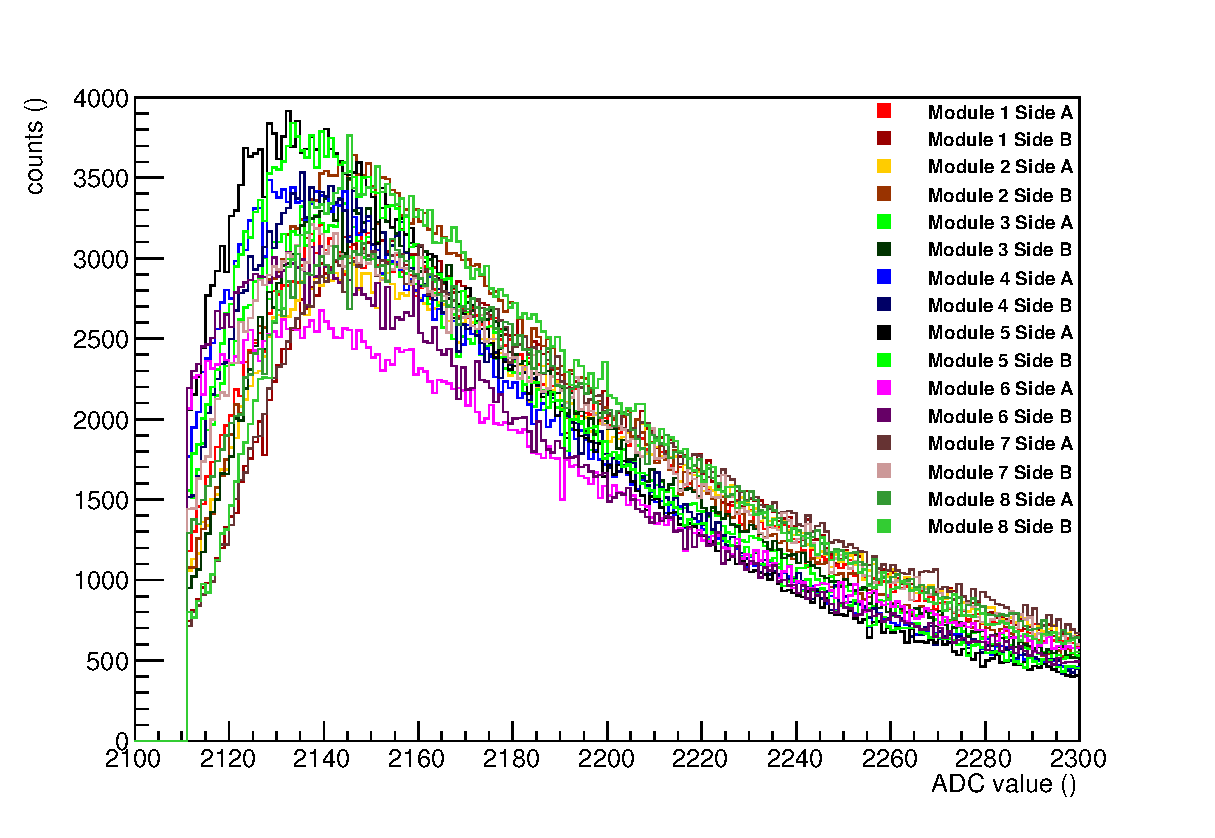
\includegraphics[width = 0.9 \textwidth]{graphics/setup/LandauPeaksRun660_old.eps}
		\caption{The landau peak at acceleration voltages around \SI{1200}{\volt}. All channels show similar width and height. Note that the threshols had to be set pretty close to the peak position as noise was a huge issue under the conditions.}
		\label{fig:allPeaksBefore}
	\end{figure}

	Later in the comissioning process, it got clear from the handbooks that the photomultiplier tubes had to be operated at accelleration voltages of \SI{1.5}{\kilo\volt} and above. To keep the singnals' height as small as possible, most of the tubes were limited to this minimal voltage, wheras the sides \todo{which ones} were set to \SI{1.6}{\kilo\volt} over showing lower rates than the others. Following this procedure, the tubes seemed much more stable and comparable, as all the gains and thresholds could now be set to the same values of \todo{enter values} and respectively, while still showing aligned peak positions \ref{fig:allPeaksAfter}. This is a huge advance to before when gains varied by a factor of almost up to four.
	
	\begin{figure}
		\centering
		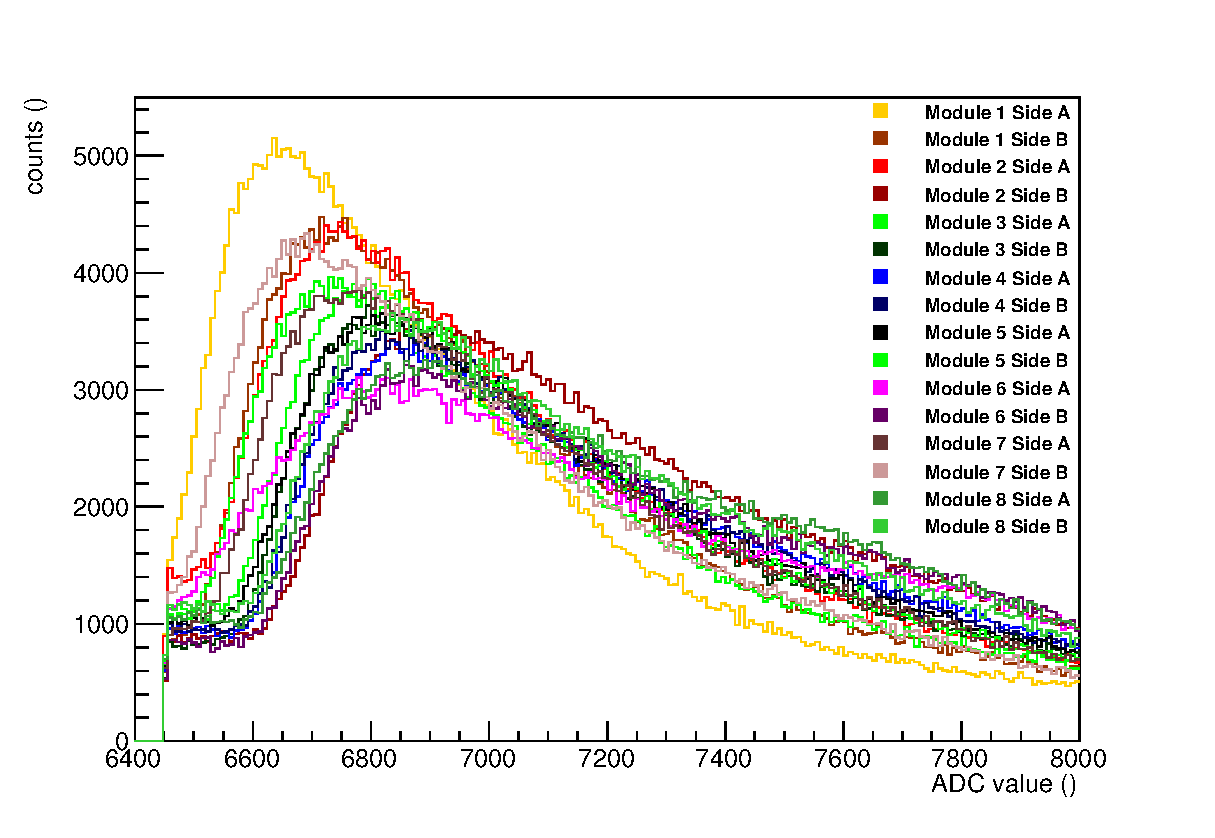
\includegraphics[width = 0.9 \textwidth]{graphics/setup/LandauPeaksRun1097_new.eps}
		\caption{Landau peaks after raising acceleration voltages. Note that this pattern was achieved solely by raising two module's side's acceleration voltages to \SI{1.6}{\kilo\volt} leaving gains and thresholds at the same level for all channels. }
		\label{fig:allPeaksAfter}
	\end{figure}



